% ---------------------------------------------------------------
% Preamble
% ---------------------------------------------------------------
%\documentclass[a4paper,fleqn,longmktitle]{cas-sc}
\documentclass[a4paper,fleqn]{cas-dc}
%\documentclass[a4paper]{cas-dc}
%\documentclass[a4paper]{cas-sc}
% ---------------------------------------------------------------

% -------------------------------------------------------------------- 
% Packages
% --------------------------------------------------------------------
% Figure packages
\usepackage{float}
\usepackage{adjustbox}
% Text, input, formatting, and language-related packages
\usepackage[T1]{fontenc}
\usepackage{subcaption}
% \usepackage[utf8]{inputenc}
% \usepackage[nomath]{lmodern}

% Margin and formatting specifications
%\usepackage[authoryear]{natbib}
\usepackage[sort]{natbib}
\setcitestyle{square,numbers}

 %\bibliographystyle{cas-model2-names}

\usepackage{setspace}
\usepackage{subfiles} % Best loaded last in the preamble

% \usepackage[authoryear,longnamesfirst]{natbib}

% Math packages
\usepackage{amsmath, amsthm, amssymb, amsfonts, bm, nccmath, mathdots, mathtools, bigints, ulem}

\usepackage{tikz}
\usetikzlibrary{shapes.geometric,angles,quotes,calc}

% --------------------------------------------------------------------
% Packages Configurations
\usepackage{enumitem}
% --------------------------------------------------------------------
% (General) General configurations and fixes
\AtBeginDocument{\setlength{\FullWidth}{\textwidth}}	% Solves els-cas caption positioning issue
\setlength{\parindent}{20pt}
%\doublespacing
% --------------------------------------------------------------------
% Other Definitions
% --------------------------------------------------------------------
\graphicspath{{Figures/}}
% --------------------------------------------------------------------
% Environments
% --------------------------------------------------------------------
% ...

% --------------------------------------------------------------------
% Commands
% --------------------------------------------------------------------

% ==============================================================
% ========================== DOCUMENT ==========================
% ==============================================================
\begin{document} 
%  --------------------------------------------------------------------

% ===================================================
% METADATA
% ===================================================
\title[mode=title]{Parameter estimation}                      
\shorttitle{Parameter estimation}

\shortauthors{A, B, C}

\author[1]{Oliwer Sliczniuk*}[orcid=0000-0003-2593-5956]
\ead{oliwer.sliczniuk@aalto.fi}
\cormark[1]
%\credit{a}

%\author[1]{Pekka Oinas}[orcid=0000-0002-0183-5558]
%\credit{b}

%\author[1]{Francesco Corona}[orcid=0000-0002-3615-1359]
%\credit{c}

\address[1]{Aalto University, School of Chemical Engineering, Espoo, 02150, Finland}
%\address[2]{2}

\cortext[cor1]{Corresponding author}

% ===================================================
% ABSTRACT
% ===================================================
\begin{abstract}
%Given a system of partial differential equations, $F(t,x,\dot{x},p,u)=0$, where $x$ represents state variables, $p$ are the parameters, and $u$ are control variables, the process model is simultaneously solved for both $x_i$ and a set of sensitivity functions, $dx_i/dp_j$, overall times $t$.These sensitivity functions measure the influence of the parameter change on the model's output. As an example, the supercritical extraction process is presented. The impact of mass flow rate, pressure, and inlet temperature on the model's output is discussed. The sensitivity analysis results prove that the considered variables can affect the extraction's yield and be used as control variables in optimization problems. Moreover, the local sensitivity analysis results are analyzed from a phenomenological point of view to enhance understanding of the process model.
Given a system of partial differential equations, $F(t,x,\dot{x},p,u)=0$, where $x$ represents state variables, $p$ are the parameters, and $u$ are control variables, we describe the supercritical extraction process. The process model describes a partially filled extractor with a fixed bed, which work under constant operating conditions. We assume that the flow is uniform across any cross-section, although the area available for the fluid phase is a function of distance. We apply the concept of quasi-one-dimensional flow to mimic the modelling of a two-dimensional case.
The collected dataset, obtained from the extraction of caraway seeds at different operating conditions, is used to estimate unknown parameters. The model-based parameter estimation applies the maximum likelihood method to estimate values of the extraction kinetic parameters such as mass partition factor, internal diffusion coefficient and radial diffusion.

\end{abstract}

\begin{keywords}
Supercritical extraction \sep Parameter estimation \sep Mathematical modelling
\end{keywords}

% ===================================================
% TITLE
% ===================================================
\maketitle

% ===================================================
% Section: Introduction
% ===================================================\section{Introduction}

\section{Introduction}
%\subfile{Sections/introduction}

\section{Materials and methods} \label{CH: Materials and methods}
%\subfile{Sections/Materials_and_methods}

\subsection{Extraction model} \label{CH: Extraction_model}
\subfile{Sections/Model}

\subsection{Low Mach number expansion}
\subfile{Sections/Low_mach_number_expansion}

%\newpage
%\section{Bayes theorem} \label{CH: Bayes}
%\subfile{Sections/Bayes_Theorem}
%\clearpage

\clearpage

\subsection{Parameter estimation} \label{CH: Parameter_estimation}
\subfile{Sections/Parameter_estimation}

\section{Results} \label{CH: Results}

\begin{figure*}[h!]
		\centering
		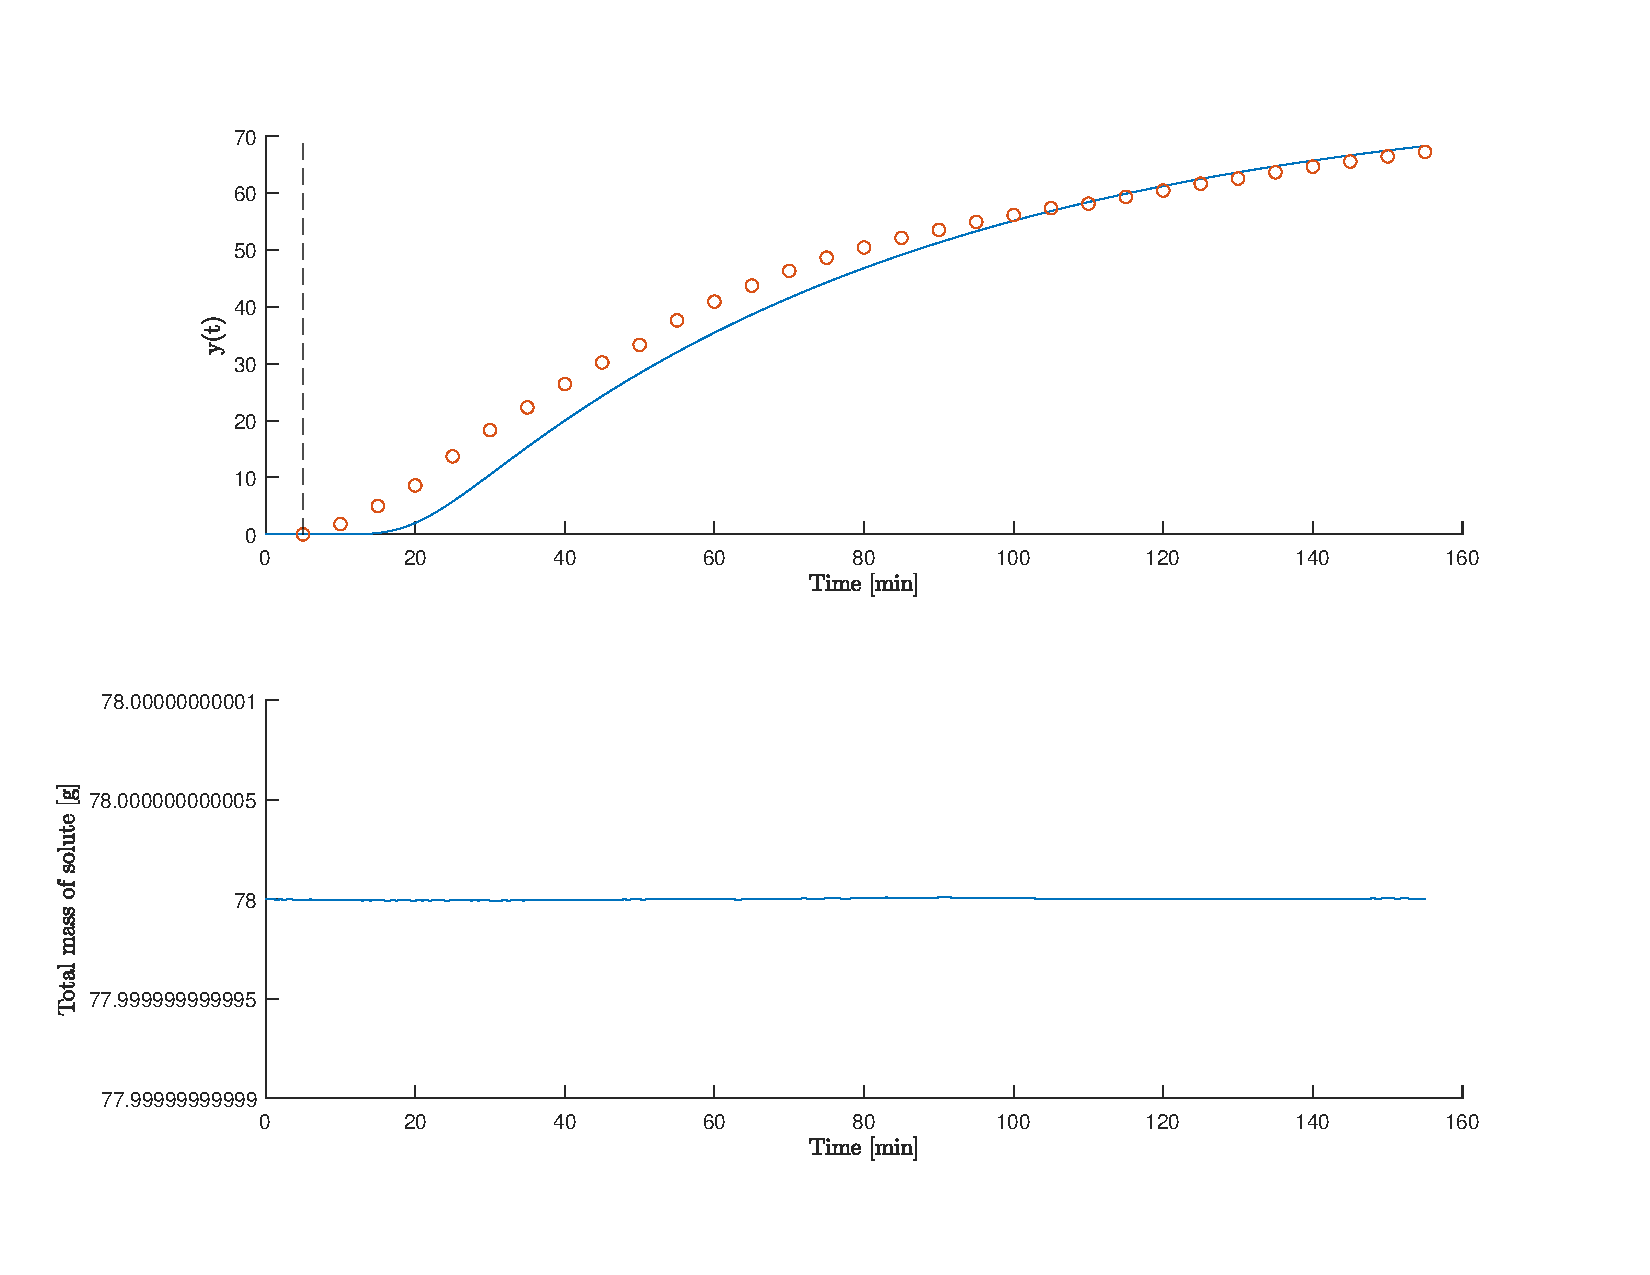
\includegraphics[trim = 0cm 0cm 0cm 0cm,clip,width=\textwidth]{Figures/Results_estimation/Yield.pdf}	
		\caption{The yield curve vs dataset}
\end{figure*}

\begin{figure*}[h!]
	\centering
	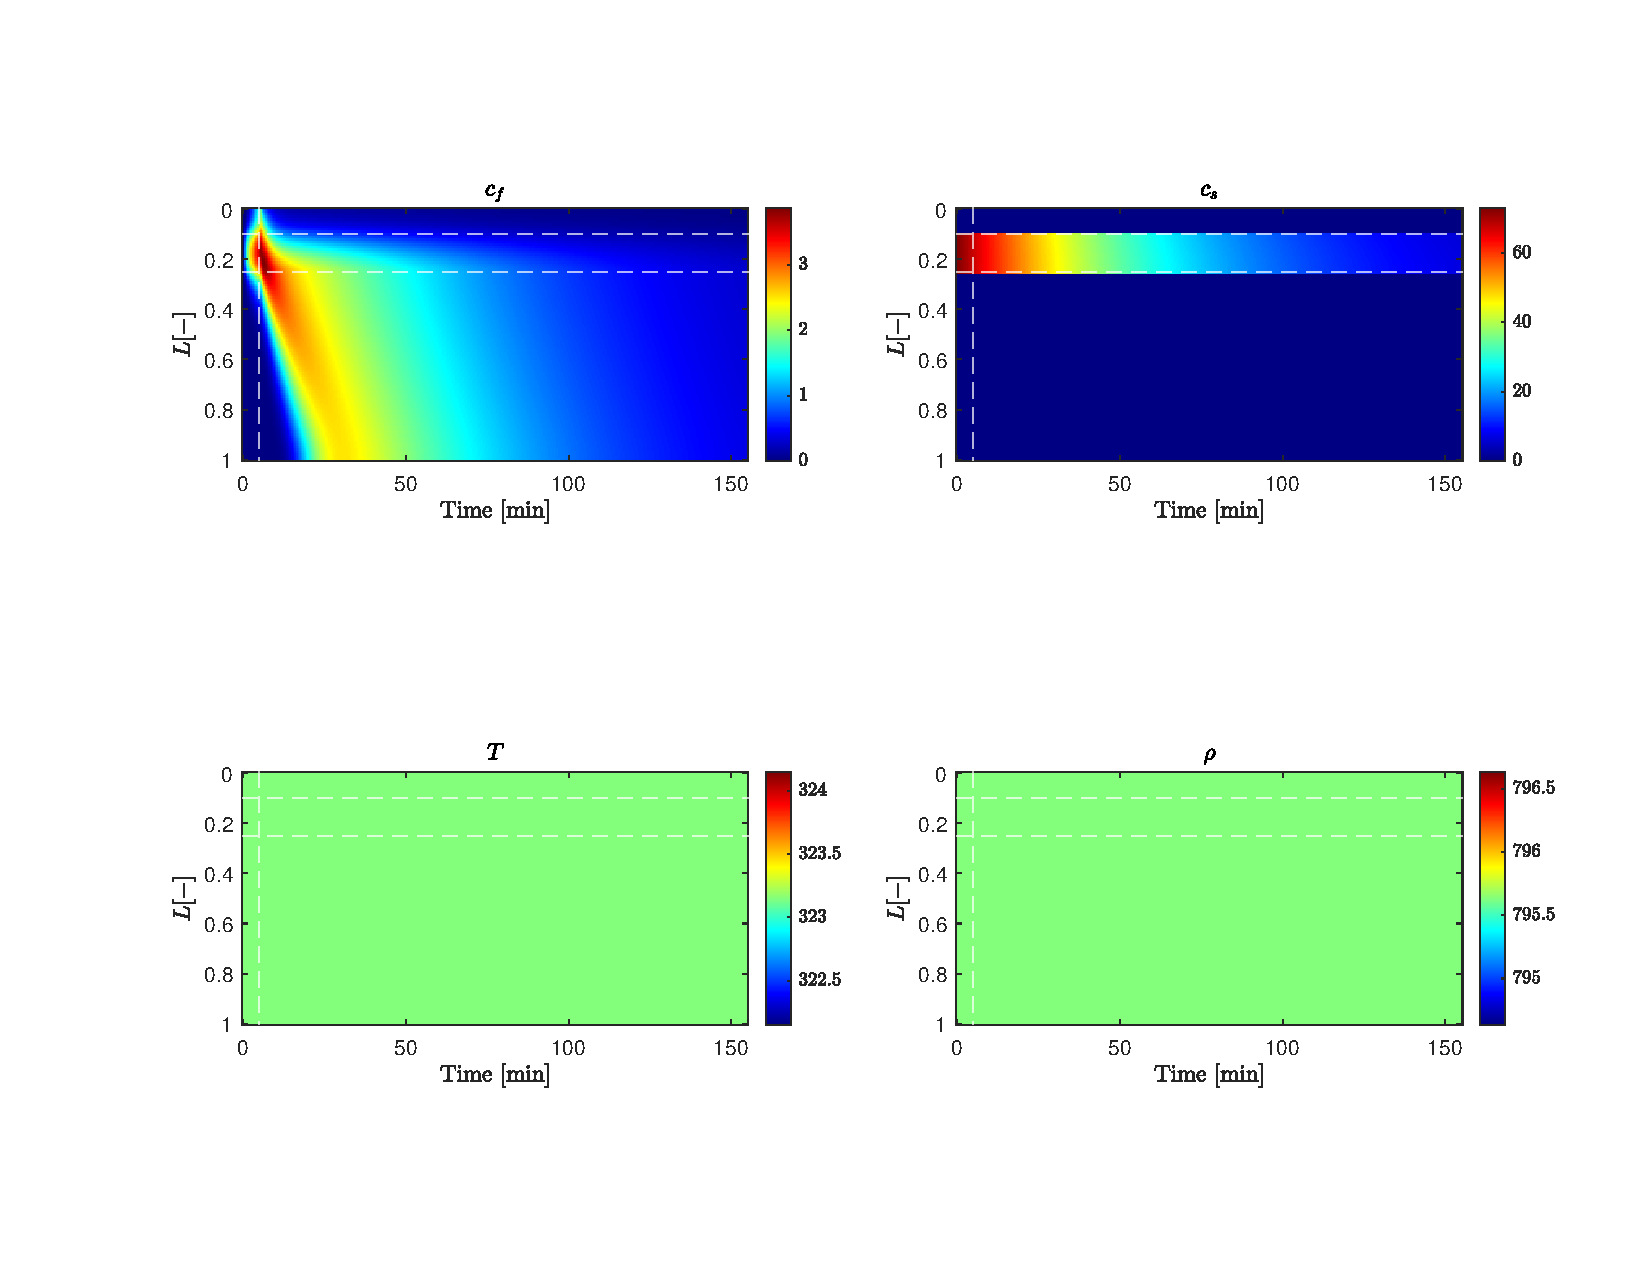
\includegraphics[trim = 0cm 0cm 0cm 0cm,clip,width=\textwidth]{Figures/Results_estimation/Profiles.pdf}	
	\caption{The fluid density based on the Peng-Robinson equation of state}
\end{figure*}

\section{Conclusions}

% ===================================================
% Bibliography
% ===================================================
%% Loading bibliography style file
\clearpage
%\bibliographystyle{model1-num-names}
\bibliographystyle{unsrtnat}
\bibliography{mybibfile}

\clearpage \appendix \label{appendix}
\section{Appendix} 
\subsection{Governing equations}
\subfile{Sections/Gouverning_equation_derivation}

\subsection{Bayes theorem} \label{CH: Bayes}
\subfile{Sections/Bayes_Theorem}

\newpage
\begin{table*}[p]
		\caption{Notation}
		\label{tab::symbols}
		\begin{tabular}{ |c|l|c| } 
			\hline
			Symbol 		& 	Description 							& Unit 						\\ \hline
			$A$			&	cross-section							& $m^2$ 					\\ \hline
			$c$			&	concentration in fluid phase			& $kg ~ m^{-3}$				\\ \hline
			$Cp$		&	specific heat of the fluid				& $J ~ mol^{-1} ~ K^{-1}$ 	\\ \hline
			$Cp_s$		&	specific heat of the solid				& $J ~ mol^{-1} ~ K^{-1}$ 	\\ \hline
			$D_e^M$		&	axial mass diffusion coefficient		& $m^2 ~ s^{-1}$			\\ \hline
			$D_e^T$		&	axial heat diffusion coefficient		& $m^2 ~ s^{-1}$			\\ \hline
			$Di$		&	internal diffusion coefficient			& $m^2 ~ s^{-1}$			\\ \hline
			$dp$		&	particle diameter						& $m$						\\ \hline
			$F(t)$		&	mass flow-rate							& $kg ~ s^{-1}$				\\ \hline
			$km$		&	partition coefficient					& $[-]$						\\ \hline
			$k^T$		&	thermal conductivity					& $W ~ m^{-1} ~ K^{-1}$		\\ \hline
			$l$			&	characteristic dimension				& $m$						\\ \hline
			$L$			&	total length of the bed					& $m$						\\ \hline
			$m$			&	mass of the oil in solid phase			& $kg$						\\ \hline
			$m_0$		&	initial mass of the oil in solid phase	& $kg$						\\ \hline
			$M_{CO_2}$	&	molecular mass of CO2					& $mol ~ kg^{-1}$			\\ \hline
			$Np$		&	number of model parameters and control variables & $[-]$			\\ \hline
			$N_{\theta}$&	number of model parameters				& $[-]$						\\ \hline
			$Nu$		&	number of control variables				& $[-]$						\\ \hline
			$Nz$		&	number of grid points in z-direction	& $[-]$						\\ \hline
			$p$			&	vector of model parameters and control variables	& $[-]$			\\ \hline
			$P(t)$		&	pressure								& $bar$						\\ \hline
			$Pe$		&	Peclet's number							& $[-]$						\\ \hline
			$q$			&	concentration in solid phase			& $kg ~ m^{-3}$				\\ \hline
			$R$			&	gas constant							& $J ~ K^{-1} ~ mol^{-1}$	\\ \hline
			$Re$		&	Reynolds number							& $[-]$						\\ \hline
			$t$			&	time									& $s$						\\ \hline
			$T$			&	temperature								& $K$						\\ \hline
			$T_0$		&	initial temperature						& $K$						\\ \hline
			$V$			&	volume of the extractor					& $m^3$						\\ \hline
			$y$			&	yield	 								& $[-]$						\\ \hline
			$z$			&	length									& $m$						\\ \hline
			$Z$			&	compressibility	factor					& $[-]$						\\ \hline
			$\epsilon$	&	void fraction							& $[-]$						\\ \hline
			$\rho$		&	density of the fluid					& $kg ~ m^{-3}$				\\ \hline
			$\rho_s$	&	solid density							& $kg ~ m^{-3}$				\\ \hline
			$\mu$		&	shape coefficient						& $[-]$						\\ \hline
			$\theta$	&	vector of model parameters				& $[-]$						\\ \hline
			$\eta$		&	viscosity								& $cP$						\\ \hline				
						& 											&							\\ \hline			
		 	Subscript	& 											&							\\ \hline
			$0$			&	initial conditions						& $[-]$						\\ \hline
			$^*$		&	equilibrium conditions					& $[-]$						\\ \hline							
		\end{tabular}
\end{table*}
\end{document}